% Author: Izaak Neutelings (September 2020)
\documentclass[border=3pt,tikz]{standalone}
\usepackage{amsmath}
\usepackage{tikz}
\usepackage{physics}
\usepackage{siunitx}
\usepackage[outline]{contour} % glow around text
\usetikzlibrary{angles,quotes} % for pic
\usetikzlibrary{calc}
\contourlength{1.3pt}

\tikzset{>=latex} % for LaTeX arrow head
\usepackage{xcolor}
\colorlet{veccol}{green!70!black}
\colorlet{pathcol}{blue!40!black}
\colorlet{xcol}{blue!70!black}
\colorlet{vcol}{green!70!black}
\colorlet{acol}{red!50!blue!80!black!80}
\colorlet{omcol}{vcol!60!black}
\colorlet{myblue}{blue!70!black}
\colorlet{myred}{red!70!black}
\tikzstyle{vector}=[->,very thick,xcol,line cap=round]
\tikzstyle{mydashed}=[dash pattern=on 2pt off 2pt]
\tikzstyle{mass}=[line width=0.6,red!30!black,fill=red!40!black!10,rounded corners=1,
                  top color=red!40!black!20,bottom color=red!40!black!10,shading angle=20]
\newcommand\rightAngle[4]{
  \pgfmathanglebetweenpoints{\pgfpointanchor{#2}{center}}{\pgfpointanchor{#3}{center}}
  \coordinate (tmpRA) at ($(#2)+(\pgfmathresult+45:#4)$);
  \draw[white,line width=0.6] ($(#2)!(tmpRA)!(#1)$) -- (tmpRA) -- ($(#2)!(tmpRA)!(#3)$);
  \draw[] ($(#2)!(tmpRA)!(#1)$) -- (tmpRA) -- ($(#2)!(tmpRA)!(#3)$);
}


\begin{document}
% CURVED PATH
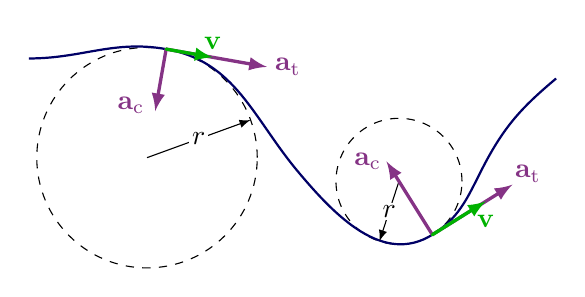
\begin{tikzpicture}
    \def\ul{0.6}
    \def\Ra{1.4}
    \def\Rb{0.8}
    \def\anga{80}
    \def\angb{-58}
    \coordinate (O1) at (0,0);
    \coordinate (O2) at (3.2,-0.3);
    \coordinate (A) at (\anga+60:1.4*\Ra);
    \coordinate (B) at ($(O1)+(\anga:\Ra)$);
    \coordinate (C) at ($(O1)!0.6!(O2)$);
    \coordinate (D) at ($(O2)+(\angb:\Rb)$);
    \coordinate (E) at ($(O2)+(\angb+70:1.4*\Rb)$);

    \draw[dashed] (O1) circle (\Ra);
    \draw[dashed] (O2) circle (\Rb);
    \draw[pathcol,thick]
    (A) to[out=0,in=\anga+90]
    (B) to[out=\anga-90,in=130]
    (C) to[out=-50,in=\angb-90]
    (D) to[out=\angb+90,in=\angb-60]
    (E) to[out=\angb+120,in=-140]++ (50:1.4);

    % POSITION
    \draw[->] (O1) --++ (\anga-60:\Ra) node[midway,fill=white,inner sep=1] {$r$}; % vector % node[midway,left=5,above right=0] {$\vb{r}$};
    \draw[->] (O2) --++ (\angb-50:\Rb) node[midway,fill=white,inner sep=1] {$r$}; % vector

    % ACCELERATION
    \draw[vector,acol]
    (B) --++ (\anga-180:0.8) node[above=2,left=0] {$\vb{a}_\mathrm{c}$};
    \draw[vector,acol]
    (B) --++ (\anga-90:1.3) node[right=-1] {$\vb{a}_\mathrm{t}$};
    \draw[vector,acol]
    (D) --++ (\angb-180:1.1) node[left=-2] {$\vb{a}_\mathrm{c}$}; %above left=-4
    \draw[vector,acol]
    (D) --++ (\angb+90:1.2) node[above right=-3] {$\vb{a}_\mathrm{t}$};

    % VELOCITY
    \draw[vector,vcol]
    (B) --++ (\anga-90:0.6) node[above=-1] {$\vb{v}$};
    \draw[vector,vcol]
    (D) --++ (\angb+90:0.8) node[below=1] {$\vb{v}$};

\end{tikzpicture}


\end{document}